\chapter{Reinforcement Learning}
\section{The Problem}
Reinforcement Learning in general is
the idea of learning from interaction with the environment;
a concept humans are familiar with albeit sometimes subconsciously.

The child learns to walk by attempts, failure,
and eventually success.
During every interaction with our environment
we are constantly aware of how it reacts to us,
be it when we walk down the street
or hold a conversation with someone.
We are even aware of animals doing the same.

\paragraph{}
The idea of trial-and-error learning has long been in play,
the term itself even used in the 19th century
to describe observations of animal behavior
\parencite{woodworth1938experimental}.

Edward Thorndike phrased the
\textit{Law of Effect}
which is,
after some of his own amendments,
still considered a basic principle
governing much of animal behavior.

\begin{displayquote}
Of several responses made to 
the same situation, those which are accompanied or closely 
followed by satisfaction to the animal will, other things being 
equal, be more firmly connected with the situation, so that, 
when it recurs, they will be more likely to recur; those which 
are accompanied or closely followed by discomfort to the ani- 
mal will, other things being equal, have their connections with 
that situation weakened, so that, when it recurs, they will be 
less likely to occur. The greater the satisfaction or discomfort, 
the greater the strengthening or weakening of the bond. 

\attrib{\cite{thorndike1911}, p. 244}
\end{displayquote}

\begin{figure}[h]
  \centering
  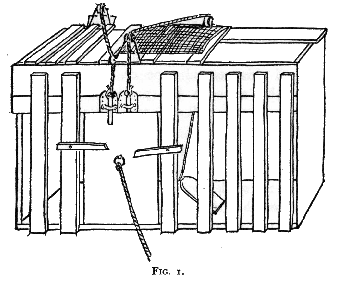
\includegraphics[width=0.7\linewidth]{puzzlebox.png}
  \caption{
    A puzzle box used by Thorndike in his experiments.
    The hungry cat is locked inside the box which it can open
    by solving some kind of puzzle
    in order to reach the fish outside.
    Results showed that the cat went from solving the puzzle by sheer happenstance
    to methodically opening it as if by habit.
  }
  \label{fig:puzzlebox}
\end{figure}

The psychological field of animal behavior and learning
has a longer history than the computational counterpart does,
with popular examples such as Pavlov's research.
The Russian Nobel laureate studied how animals
responded to different stimuli:

\begin{displayquote}
It is pretty evident that under natural conditions the normal animal must
respond not only to stimuli which themselves bring immediate benefit or harm,
but also to other physical or chemical agencies—waves of sound,
light, and the like—which in themselves only signal the approach of these stimuli;
though it is not the sight and sound of the beast of prey 
which is in itself harmful to the smaller animal, but its teeth and claws.
\attrib{\cite{pavlov1927conditional}, p. 14}
\end{displayquote}

In this same text the term "reinforcement"
was used for the first time in the context of animal learning.

Pavlov is most known for his experiment with dogs.
He noticed dogs would produce saliva in response
to receiving food.
He then associated a secondary stimulus to the act
of feeding the animals
by ringing a bell beforehand.
The dogs learned to associate the bell
with food and produced saliva
upon hearing the bell,
even before or without receiving anything.

\paragraph{}
Using trial-and-error to achieve artificial intelligence 
was among the earliest ideas in the field.
Alan Turing describes positive and negative stimuli
to influence an algorithm:

\begin{displayquote}
  When a configuration is reached for which the action is undetermined, a
random choice for the missing data is made and the appropriate entry is
made in the description, tentatively, and is applied. When a pain stimulus
occurs all tentative entries are cancelled, and when a pleasure stimulus
occurs they are all made permanent.

\attrib{\cite{turing1948intelligent}}
\end{displayquote}

Reinforcement Learning as I treat it here
solely means the computational approach
to learning from interaction,
except where mentioned explicitly.
We will not theorize on animal behavior
or try to model it in order to create computational models.
Sometimes, however,
inspiration is drawn from animal behavior
but it usually is no more than that;
analogies only go as far as they serve us.
The perspective used here is that of the engineer,
not the neuroscientist.

\paragraph{}
Central to reinforcement learning is that a learner
interacts with its environment in order to learn
and ultimately aims to achieve some goal.
Applied to human behavior in the course of a lifetime,
we could say humans -in general- try to optimize happiness.
Applied to something less daunting than the human condition,
a sculptor may try to optimize beauty
or expressivity of a sculpture,
learning along the way how to do so in the best possible way.
It is this goal-based interaction that forms the core
to reinforcement learning.

\paragraph{}
Reinforcement learning can be characterized
by three distinguishing features,
setting it apart from other fields of learning

\begin{description}
  \item[Closed loop]
    In order to learn, a learning agent must interact
    with the environment to collect the necessary information.
    However, each action changes the environment in a certain way
    and in turn influences the agent's future inputs.
    This forms a \textit{closed loop}.

  \item[Discovery]
    An agent is provided with no instructions on what actions to take
    and how this will impact the environment.
    It is to discover this itself.

  \item[Time factor]
    Consequences of an action can be delayed by an unknown amount of time.
    Even the reward signal can be received many time steps later.
    The agent is to figure out for itself
    how its actions relate temporally to consequences.
    
    A good example of this is the game of chess with only a reward signal
    at the end of a match, either positive or negative.
    Some moves during the game are probably more important
    than others and some more complicated,
    like traps that take multiple moves to set up.
    Yet all moves together are rewarded with only a single signal
    at the end of the match.
    It is for the agent to unravel and attribute
    its actions according to importance.
\end{description}

\subsection{Reinforcement Learning and Machine Learning}
As I tried to convey above,
a crucial aspect to reinforcement learning
is trial-and-error, learning from interactions
with an environment that is not necessarily known.
This makes reinforcement learning different from
\textit{supervised learning}
which is most associated with machine learning.
In a supervised setting,
a labeled example set is provided
for the learner to learn from.
Learning in this context means generalizing from the training set
so queries about data not in this set
can still be answered accurately.

Reinforcement learning is different
in that it takes on more of the problem;
a learning algorithm is not presented with data
but instead must gather it by interacting with the environment.
In doing so it must also make a tradeoff between exploration and exploitation,
a characterizing element to reinforcement learning.
A learning agent can either \textit{exploit}
what it knows to be the best action in order to achieve its goal,
thereby possibly ignoring alternative routes of action
that would have resulted in better results,
or choose to \textit{explore}
what impact its actions have on the environment.
Neither strategy can be followed exclusively
if one wants to learn anything worthwhile,
a good combination of both is always needed.

\paragraph{}
On the "opposite" side of supervised learning
is we call unsupervised learning,
which is about finding hidden patterns in unlabeled data.
The supervision gap between the two obviously pertains
to whether the data has been created in a supervised manner.
An illusion is created that there are two sides to machine learning,
though reinforcement learning does not seem to fit either.
Reinforcement learning is effectively a third machine learning paradigm.

\subsection{Applications (TODO)}
Reinforcement learning has been applied in a multitude of domains,
not only the ones immediately called to mind when thinking
of autonomous agents like physical robots of all kinds,
though those have definitely gained a lot of attention.

%TODO pff geen zin nu
\paragraph{}
Survey by \cite{Kober2013}

\paragraph{}
Talk about self-driving cars

With the surge of new techniques and faster machines
reinforcement learning has also gotten popular with the public.
%TODO self-driving cars


\section{Reinforcement Learning Framework}
There are only few components to the reinforcement learning problem.
The learner and actor is dubbed the agent and everything outside it the environment.
The agent perceives its environment and acts on it,
receiving a reward in return.
The latter is a numerical value
which the agent tries to gain as much as possible of
during its time interacting with the environment.
This interaction goes on continually:
observation followed by action followed by reward.
The goal of the agent is to maximize its accumulated reward
over the entire span of a task,
i.e. an instance of a problem.
In order for it to do so
it must learn to not only look to immediate rewards
but must also look to what the future has to offer.

\begin{figure}[h]
	\center
	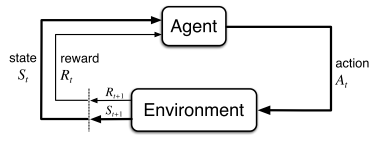
\includegraphics[width=.5 \linewidth]{agent-environment.png}
	\caption{The agent interacts with the environment and consequentially perceives a reward and the next state of the environment.}
	\label{agent-env}
\end{figure}

Formally, we divide the problem into discrete time steps $t$.
A time step occurs every time the agent perceives a state $s_t$
from the set of possible states $\mathcal{S}$.
Based on this state the agent selects an action $a_t$
from its repertoire of actions $\mathcal{A}(s_t)$
available to it at in state $s_t$.
As a result, the next step it will receive a numerical reward $r_{t+1}$
along with the next state $s_{t+1}$,
and so on and so on.

As you can see, the problem setting is entirely abstract
and can be filled in in various ways.
In fact, the same practical problem may be defined in different ways
depending on the goal.
A state could just as well represent a robot's raw sensor readings
as well as higher-level representations
such as whether it's looking at a green or red light.
We say that state is provided by the environment
even though one could argue a robot's sensors
are part of the agent.
Instead, we look at the agent as the observer and decision-maker
taking in everything from a distance,
even its physical body external to it
as part of the environment.
Similarly to states,
actions can range from raw low-level values
like motor voltages
to higher-level concepts like which room to go to
or whether to turn left or right.
Basically, actions are decisions taken by the distant observer,
for the designer to decide which shape they take.

\section{Markov Decision Processes}
The Markov property is an interesting property for a problem to have
because it states that all relevant information at some point
is present in a state.
This means that the whole history leading up to a certain point,
insofar that it is relevant,
is encoded in the state at that time. 
Such a state is said to be Markov.

Formally, consider the probability of ending up in a state $s_{t+1}$
with reward $r_{t+1}$
after performing some action $a_t$
in a state $s_t$.
This probability is denoted

$$Pr(s_{t+1}=s', r_{t+1}=r | s_t, a_t)$$

We would say a state signal is Markov if this probability is the same as

$$Pr(s_{t+1}=s', r_{t+1}=r | s_t, a_t, s_{t-1}, a_{t-1},..., s_0, a_0)$$

which is the same scenario except given the entire state and action history. If these two are indeed equal, then the history is effectively encoded in the current state $s_t$.

\paragraph{}
START on mdp's here

\section{Value Functions}

\section{Temporal Difference Learning}

\section{Q-Learning}
Often we will discount future rewards
by a certain factor $\gamma$ per time step,
resulting in a total future discounted return
for the agent of
$R_t = \sum{T}{t'=t} \gamma^{t'-t}r_{t'}$,
with T the last time step.
This return is dependent on some policy $\pi$.
We now define $Q*(s,a)$ as the maximum expected return
when in a state s and taking action a.
This assumes we already know the optimal policy
in every subsequent state.
More formally,
$Q*(s,a) = max_{\pi}E[R_t|s_t=s, a_t=a, \pi]$

\paragraph{}
Since we assume we already know the optimal action in every state,
$$Q*(s,a) = E_{s'~\mathcal{E}}[r+\gamma max_{a'}Q*(s',a')|s,a]$$

Q-learning uses this equation directly
by plugging it into an iterative update.
Every step, the known Q-value for the visited state-action pair
is updated using a simple update rule:

$$<<TODO Q-learning update rule>>$$

with $\alpha$ a discount factor to stabilize the update.
This learned action	-value function directly approaches
the optimal action-value function $Q*$,
meaning that it always learns the optimal policy
of taking action $a' = argmax_{a}Q(s,a)$
in any state s.
The policy that is used to learn these Q-values
is only used for exploration purposes such that
sufficient state-action pairs are visited
and updated.
However, the policy itself is not optimized.
We call this off-policy learning,
as opposed to on-policy learning such as Sarsa-TD
where Q-values are updated with respect to
the currently used policy.
An advantage of Q-learning
is that it is guaranteed to converge
with probability 1
once certain conditions are fulfilled,
such as sufficiently small step size $\alpha$.

\paragraph{}
A problem with this learning approach is that
it enumerates all state-action pairs,
without generalization beyond visited pairs
and the added disadvantage of having to visit
each state-action pair multiple times
in order to have the Q-values converge.
Note that this makes the exploration strategy especially important,
as an agent that starts with a default Q-value assumption of 0
for each state-action pair can easily overfit
to non-zero Q-values if it is too greedy.
Moreover, and most importantly,
this approach does not scale well beyond only the smallest and most trivial
of state-action spaces.
This because the agent won't be able to enumerate all state-action pairs
sufficiently in such scenarios.
In the next section I will discuss how to alleviate this problem.

\section{Function Approximation}
To combat the problems brought along by a large state-action space,
we can use function approximators instead of storing Q-values
for each state-action pair,
which would quickly become infeasible.
To this end,
we could use any approximation method commonly used in machine learning
to approximate our state-action values.
However, reinforcement learning makes some methods
less suitable than others.
Samples gathered iteratively using reinforcement learning
usually have high correlation since an agent
takes a certain path through
the state-action space,
where neighboring states are usually somewhat similar.
The target to be learned is also not stationary,
since the real target value is often now known
but bootstrapped with some estimation.
For example,
in Q-learning the optimal action-value function $Q*$
is approximated using $r+\gamma max_{a'}Q(s',a')$
since we do not know the optimal $Q*$ in advanced.
This substituted target is still changing
because it has not been learned fully yet
and is both the value to be learned
as the target used for learning.
In subsequent sections I will discuss
how we can minimize the impact of these problems.
Still, it is important to be aware of them
when designing a function approximator.

\paragraph{}
One way of looking at the error of a Q-value approximator
with parameters $\theta$ is to look at the Mean Squared Error
between between the maximum expected return and
the predicted state-action value for all state-action pairs:
% formula kinda from sutton
% https://webdocs.cs.ualberta.ca/~sutton/book/ebook/node86.html
$$MSE(\theta) = \sum_{s \in S}[Q*(s,a)-Q(s,a,\theta)]^2$$
This error can then to be minimized over all samples
by a method such as gradient descent.

That is the traditional machine learning approach.
Note that reaching a global optimum for the parameters
is often only possible for linear functions
and not so anymore for more complex nonlinear functions.
In the harder case, we could instead look for local optima,
i.e. a case when $MSE(\theta') < MSE(\theta)$
for all $\theta$ near $\theta'$.

One should also be careful with simply minimizing the MSE
of the state-action function approximator
as our ultimate goal is to have the best policy $\pi$,
% TODO so.. do they collide? Sutton was vague at first	
two goals that do not necessarily collide.


\section{Eligibility Traces}
Valt te overwegen.
